
%(BEGIN_QUESTION)
% Copyright 2008, Tony R. Kuphaldt, released under the Creative Commons Attribution License (v 1.0)
% This means you may do almost anything with this work of mine, so long as you give me proper credit

Her vises en sekantlinje og en tangentlinje (begge tynne) til en kurve (tykk):

$$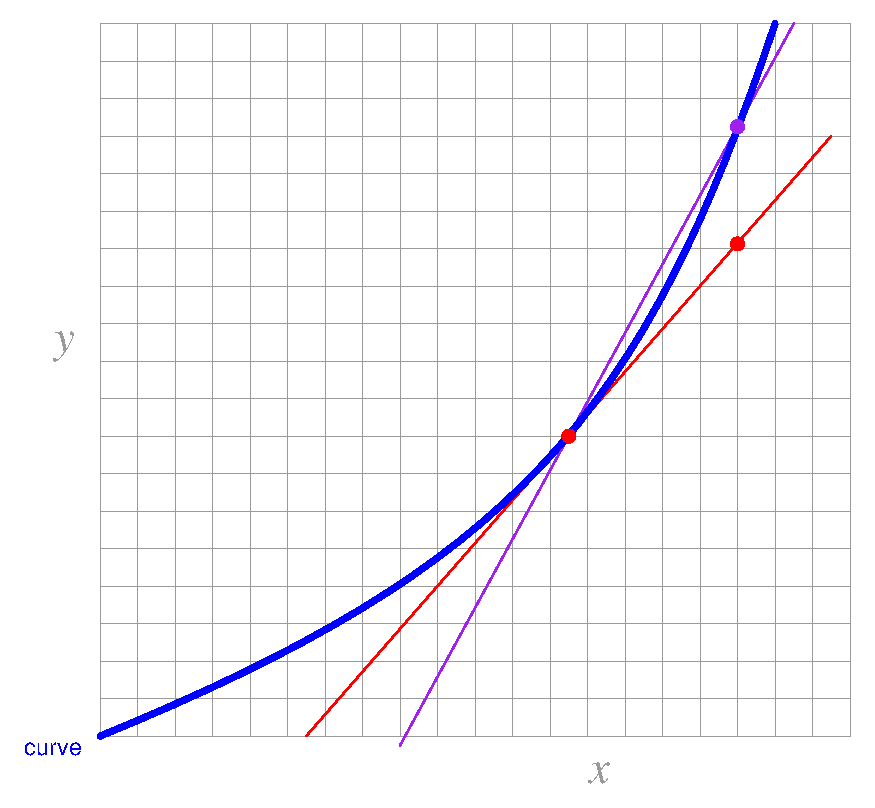
\includegraphics[width=15.5cm]{i01508x01.eps}$$

Helningen til én av disse linjene representeres av forholdet mellom to ``inkrementer,'' $\Delta y$ og $\Delta x$:

$${\Delta y \over \Delta x}$$

\vskip 10pt

Helningen til den andre linjen representeres av forholdet mellom to ``differensialer,'' $dy$ og $dx$, bedre kjent som en {\it derivert}:

$${dy \over dx}$$

\vskip 10pt

Bestem hvilken helning ($\Delta y \over \Delta x$ eller $dy \over dx$) som hører til hvilken linjetype (sekant eller tangent), og merk alle inkrementer og differensialer i grafen.

\underbar{file i01508}
%(END_QUESTION)





%(BEGIN_ANSWER)

$$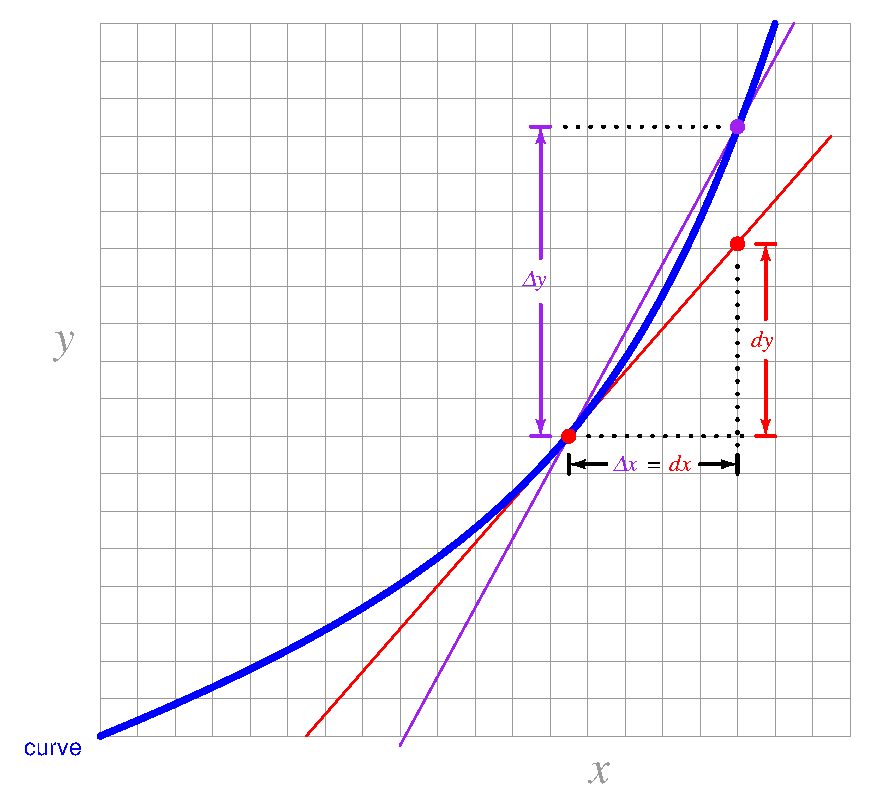
\includegraphics[width=15.5cm]{i01508x02.eps}$$

$${\Delta y \over \Delta x} = \hbox{ Helning til sekantlinje}$$

\vskip 10pt

$${dy \over dx} = \hbox{ Helning til tangentlinje}$$

\vskip 10pt

På grunn av den klassiske definisjonen av den deriverte som grensen for sekantlinjens helning når $\Delta x$ går mot null, tror mange i starten at $dx$ og $dy$ nødvendigvis må være svært små. Slik er det ikke. Differensialer som $dx$ og $dy$ kan ha enhver ikke-null reell verdi; poenget er at de angir helningen til tangentlinjen, ikke helningen til kurven mellom intervaller. For praktiske anvendelser av store differensialverdier, se en innføringsbok i kalkulus om {\it lineære tilnærminger} med differensialer.

%(END_ANSWER)





%(BEGIN_NOTES)


%INDEX% Mathematics, calculus: derivatives and tangent lines
%INDEX% Mathematics, calculus: incremental ratios and secant lines

%(END_NOTES)

